
Query processing refers to the range of activities involved in extracting data from a database.
These activities include the translation of queries from high-level languages into formats that can be processed
by the database, query-optimizing transformations, and actual evaluation of queries.

Query processing has been studied extensively in the context of relational database systems.
Relational databases provide sophisticated querying capabilities and require complex query processing techniques
to connect declarative query languages to efficient query execution.

On the other hand, databases that belong in the class of nonrelational database systems (also referred to as NoSQL)
in general make design decisions that favor scalability (very large datasets or very high write throughput) over rich
query models, often supporting only primary key lookups.
There, query processing is mainly linked to data distribution schemes and involves the use of secondary indexes.

The purpose of this chapter is to present an overview of several ``textbook'' query processing techniques.
Our work is influenced by and builds on top of the techniques presented in this chapter.

\section{Query Processing in Relational Database Systems}

The database component responsible for query processing is the \textit{query processor}.
The role of a relational query processor is, given a declarative high-level statement (often SQL), to validate it,
optimize it into a procedural dataflow execution plan, and execute that dataflow program.

Query processing consists of the following phases \cite{hellerstein:databasearchitecture, kossmann:distqeuryprocessing}:

\bigskip
\noindent
\textbf{Query Parsing.}
The goal of the query parsing is to translate a given query into an internal representation that can
be processed by later phases, commonly a tree of relational operators \cite{silberschatz:dbbook}.
In generating the internal form of the query,
the query processor checks the syntax of the given query,
verifies that the relation names that appear in the query are valid names of relation in the database,
and verifies that the user is authorized to execute the query.

\bigskip
\noindent
\textbf{Query Rewrite.}
In the query rewrite phase, the query processor transforms the query in order to carry out optimizations that are
beneficial regardless of the physical state of the system
(the size of tables, presence of indices, locations of copies of tables etc.)

Typical transformations include:
\begin{itemize}

  \item \textbf{Elimination of redundant predicates and simplification of expressions:}
  This includes the evaluation of constant arithmetic expressions,
  short-circuit evaluation of logical expressions via satisfiability tests,
  and using the transitivity of predicates to induce new predicates.
  Adding new transitive predicates increases the ability of the following phase (query optimization) to construct query
  plans that filter data early in execution, and make use of index-based access methods.

  \item \textbf{View expansion, sub-query un-nesting:}
  For each view reference that appears in the query, the query processor retrieves the view definition and rewrites the
  query to replace that view with its definition.
  In addition, this phase flattens nested queries when possible.

  \item \textbf{Semantic optimization:}
  In many cases, integrity constrains defined by the schema can be used to simplify queries.
  An important such optimization is redundant join elimination (for example, a query that joins two tables but does not
  make use of the columns of one of the tables).

\end{itemize}

\bigskip
\noindent
\textbf{Query Optimization.}
In the query optimization phase, the optimizer (the query processor component responsible for query optimizations)
transforms the internal query representation into an efficient plan for executing the query.

A query plan can be thought of as a dataflow diagram that specifies how the query is to be executed.
A common approach to represent a query plan is using a tree:
the tree's nodes are operators
--- each operator carrying out a particular operation such as join, group by, sort, scan, etc. ---
and edges represent consumer-producer relationships between operators.

The optimizer is responsible for decisions such as which indices to use to execute a query,
which methods to use to execute the operators of a query,
and in which order to execute a query's operations.
In a distributed system, the optimizer also decides at which node each operation is to be executed.

Selinger et al.’s foundational paper on System R \cite{selinger:systemr} decomposes the problem of query optimization
into three distinct sub-problems: cost estimation, relational equivalences that define a search space, and cost-based
search.
The optimizer assigns a cost estimate to the execution of each component of a query, measured in terms of I/O and CPU
cost.
To do so, the optimizer relies on pre-computed statistics about the contents of each relation, and heuristics for
determining the cardinality of the query output.
It then uses a dynamic programming algorithm to construct a query plan based on these cost estimates.

\bigskip
\noindent
\textbf{Query Execution}
Query execution is carried out by the \textit{query execution engine}.
The query execution engine is the query processor's component that provides implementations for every operator.

The most common approach used to implement query operators is the iterator model \cite{graefe:queryevaluation}.
Iterators can be described using the object-oriented paradigm.
Figure~\ref{lst:iterator} shows a simplified definition for a general iterator class.

\begin{lstlisting}[caption={Iterator class pseudocode \cite{hellerstein:databasearchitecture}},label={lst:iterator},captionpos=b,language=Java]
class iterator {
  iterator &inputs[];
  void init();
  tuple get_next();
  void close();
}
\end{lstlisting}

The iterator model has certain useful properties for modeling query execution:
\begin{itemize}

  \item All iterators have the same interface.
  As a result, a consumer-producer relationship can exist between any two iterators, and thus, any plan can be executed.
  In addition, the common interface means that each iterator's logic is independent of its children and parents in the
  graph.

  \item Τhe iterator paradigm supports pipelining of results from one operator to another.

\end{itemize}

\subsection{Materialized Views}

An important element of the relational model is the \textit{view}.
A view is a ``virtual relation'' defined by a query that conceptually contains the result of that query.
Views are not precomputed and stored; the database stores only the query defining the view.
Each time the view is used, the database expands it on the fly into the underlying query,
and then processes the expanded query.

In contrast, a materialized view is a view whose contents are computed and stored by the database.
In many cases reading the contents of a materialized view is much more efficient than computing the contents of the view
by executing the query that the view defines.
Essentially, a materialized view is a precomputed cache of query results.
The use of materialized views is a common technique for reducing query response time.

\subsubsection{View maintenance}

An important aspect of materialized views is that when the data referred in the view definition changes,
the view must be kept up-to-date.
A simplistic way of achieving this to recompute the materialized view on every update.
A better option is to, on each update, modify only the affected parts of the view.
This approach is known as incremental view maintenance.
There is considerate research on incremental view maintenance for in relational databases
\cite{larson:outerjoinviewmaintenance, lee:multiplejoinviewmaintenance, zhuge:viewmaintenance}.

Another design decision when incremental view maintenance is used, is when to perform the maintenance:
in \textit{synchronous} view maintenance, view maintenance is performed as soon as an update occurs,
as part of the updating transaction,
while in \textit{asynchronous} or lazy view maintenance,
updating the view is deferred to a later time \cite{zhou:lazymvMaintenance}.
Materialized views with deferred view maintenance may not be consistent with the underlying data.

\subsubsection{Query Optimization and Materialized Views}

Materialized views add further consideration to query optimization:

\begin{itemize}

  \item Rewriting queries to use materialized views.
  The query processor may produce a more efficient query plan by rewriting the query to make use of an available
  materialized view.

  \item Replacing the use of a materialized view with its definition.
  It may sometimes be beneficial to replace a materialized view with its definition, if the view does not have any
  indices that can be used to speed up the query, but the underlying relations do.

\end{itemize}

\subsubsection{Materialized View Selection}

Materializing an appropriate set of views and processing queries using these views can significantly speed up
query processing since the access to materialized views can be much faster than recomputing the views.
In principle, materializing all queries that a system may receive can achieve the optimal query response time.
However, maintaining a materialized view incurs a maintenance cost.
In addition, query results may be too large to fit in the available storage space.
There is therefore a need for selecting a set of views to materialize by taking into account query processing cost,
view maintenance cost and storage space.
The problem of choosing which views to materialize in order to achieve a desirable balance among these three
parameters is known as the view selection problem \cite{gupta:viewselection, mami:viewselection}.

\subsection{Caching}
Another technique for speeding up queries, besides the use of indexes and materialized views, is caching:
storing the result of a costly computation so that repeated reads of this result can be performed without re-executing
the computation, if the underlying data has not change.

A common approach is to deploy a \textit{caching tier} between the database system and the clients.
In-memory key-value stores such as Redis \cite{redis:cache} and memcached \cite{memcached:wiki} are often used for this
purpose.

However, this approach requires application logic to invalidate or replace cache entries,
which may be complex and error prone.

\subsection{Distributed Query Processing}

So far we covered query processing from the perspective of a single-node database, without considering data distribution.
However, data is inherently distributed \cite{bacon:spanner, cockroachdb:docs} and therefore query processing needs to
efficiently operate on distributed data.
In addition, query processing computations need to be able to be distributed and run in parallel on multiple nodes to
achieve better scalability.

In Ingres \cite{epstein:ingres}, relations can be distributed across a collection of ``sites''.
Query processing is based on \textit{decomposing} queries into sub-queries that can be processed on a single site.
The database uses query decomposition heuristics based on two optimization criteria:
minimizing response time and minimizing network traffic.

Spanner \cite{bacon:spanner} is sharded, geo-replicated relational database system.
Spanner uses a \textit{distributed union} operator in the query tree to represent query distribution.
Distributed union is used to a sub-query to each shard of a table, and concatenate the results.
It provides a building block for more complex distributed operators such as distributed joins between independently
sharded tables.

When a query tree is initially created, a distributed union operator is inserted immediately above every table.
In the query optimization phase, where possible, query tree transformations may pull the distributed union operator up
the tree in order to push the maximum amount of computation to the servers.
In the query execution phase, distributed union routes a sub-query request addressed to a shard, to one of the nearest
replicas of that shard in order to minimize latency.

CockroachDB employs an mechanism for distributed query processing \textbf{computation} \cite{cockroachdb:distsql}
(for example join, aggregation, or sorting) on multiple nodes in order to improve performance.
In CockroachDB, a query plan is a tree of operators, termed \textit{aggregators}:
each aggregator consumes an input stream of records and produces an output stream or records.
The key idea is that an aggregator splits the input stream into \textit{groups}:
the computation for each group is independent of the computation for other groups; the output stream is the
concatenation of computation result for all groups.
Since results for each group are independent, different groups can be processed on different nodes.


\section{Query Processing in Non-Relational Database Systems}

The querying capabilities of a non-relational database mainly follow from their distribution model and data model.
Thus different non-relational databases have varying querying capabilities.

To further discuss query processing in non-relational databases,
we first briefly introduce the data models and data distribution techniques used in these systems.

\subsection{Non-relational Database Data models}
\noindent
\textbf{Key-Value Stores.}
A key-value store's data model is a map/dictionary of key-value pairs.
As the structure of values is opaque to the database system, this data model only supports get and put operations
(requesting and writing value using a key).
Key-value stores in generally favor scalability over a richer data model and more complex query capabilities:
the simple key-value model makes partitioning and locating data efficient, thus enabling these systems to achieve low
latency and high throughput.

\bigskip
\noindent
\textbf{Document Stores.}
A document store is a key-value store that restricts values to semi-structured formats such as
XML, YAML, JSON or BSON \cite{bson:spec}.
This enables more sophisticated data access capabilities:
apart from retrieving an entire document from its key, documents stores support predicate queries
(retrieving the keys of all documents that match a given predicate), and joins.

\bigskip
\noindent
\textbf{Wide-column Stores.}
The data model of wide-column stores is often depicted as a relational table with many sparse columns.
More accurately, this data model can be described as a distributed, multi-level, sorted map.
The first-level keys identify rows (row keys) and the second-level keys identify columns (column keys).
In some wide-column stores multi-versioning is implemented by adding third-level, timestamp keys.

\subsection{Partitioning}
\label{sec:partitioning}

Partitioning is data distribution technique, in which the records of a database are split into subsets called partitions
so that different partitions can be assigned to different nodes (also known as sharding).

The goal of partitioning is to spread data and load evenly across nodes.
When implemented efficiently, it enables horizontal scaling:
doubling the number of nodes in the system should make the system able to handle double the volume of data, and
should double the system's read and write throughput.

The sharding techniques commonly used in non-relational databases are range and hash partitioning.

\bigskip
\noindent
\textbf{Range partitioning.}
Range partitioning assigns a continuous range of keys to each partition.
These ranges of key are not necessarily evenly spaced, because data may not be evenly distributed.
Partition boundaries might be chosen manually by an administrator, or automatically by the database.

Within each partition keys are kept in sorted order.
This has the advantage that range queries on the partitioning key are efficient:
it is easy to determine which partitions contain keys of a given range, and within each partition the key can be treated
as an index.

The downside of this partitioning scheme is that certain access patterns can lead to hotspots.
Therefore, systems that use range partitioning need mechanisms for detecting and resolving hotspots.

Range partitioning is used by Bigtable and its open source equivalent HBase \cite{hbasebigtable:comparison},
RethinkDB, and MongoDB before version 2.4.

\bigskip
\noindent
\textbf{Hash partitioning.}
An alternative approach that avoids the risks of skew and hotspots is to use a hash function to determine the partition
for a given key.
Hash partitioning assigns each partition a range of hashes --- rather than a range of keys --- and every key whose hash
falls within a partition's range is handled by that partition.

This partitioning scheme is efficient at distributing keys fairly among partitions.
The downside of this approach is that does not allow for efficient range queries,
as adjacent keys are scattered across multiple partitions.

Hash partitioning is used in Amazon's Dynamo, MongoDB since 2.4 \cite{mongo:hashpartitioning}, Riak, CouchBase,
and Voldemort.

\subsection{Replication}
\label{sec:replication}

Partitioning is usually combined with replication so that copies of each partition are stored on multiple nodes.
Replication improves availability by allowing the systems to continue working even if some of its parts have failed,
and increases read throughput by increasing the number of machines that can serve read queries.

Considering a single partition, each node that takes part in the replication, called a replica, stores a copy of the
partition.
A replication strategy answers two design decisions:
when a write request is send to the database (1) in which replica the write is accepted,
and (2) when the corresponding data changes are propagated to other replicas \cite{gray:replication}.

\bigskip
\noindent
A common approach to the first design decision is called \textit{leader-based} replication.
One of the replicas is designated the \textit{leader} (also termed \textit{master} or \textit{primary}).
Every write is sent to the leader.
The leader determines the order in which writes should be processed,
and sends the corresponding data changes to the other replicas
(termed \textit{followers}, \textit{slaves} or \textit{secondaries}),
Followers apply those changes in the same order.
Reads can be performed either from any replica.

This approach is used in MongoDB, RethinkDB, and Espresso.

Leader-based replication has one main downside:
as there is only one reader (when replication is combined with partitioning there is one leader per partition),
and all database writes must go through it, if the leader is unreachable writes cannot be performed.

An extension of leader-based replication is to allow more than one replicas to accepts writes.
In \textit{multi-leader} replication there are multiple readers,
each processing writes and forwarding the corresponding data changes to all other replicas.
Each leader acts also as a follower to the other leaders, accepting writes from them.

An alternative approach, termed \textit{leaderless} replication,
is to allow any replica directly accept writes from clients.
Each write is sent (either by the client, or by a coordinator) to $W$ replicas, and each read is sent to $R$ replicas,
where $W$ and $R$ are configuration parameters.
In order to ensure that eventually all data is propagated to every replica,
leaderless replication implementations often employ two mechanisms:
(1) read repair, a way to detect and update stale values during reads,
and (2) anti-entropy, having a background process that replicates missing data between replicas.

This approach was popularized by Amazon's Dynamo.
Riak, Cassandra, and Voldemort are datastores with leader replication models inspired by Dynamo.

\bigskip
\noindent
There are two approaches for the design decision ``when the leader propagates data changes to followers''.
In \textit{synchronous} (or \textit{eager}) replication the leader propagates changes synchronously
and waits for acknowledgements from followers before reporting success to the user.
In \textit{asynchronous} (or \textit{lazy}) replication the leader propagates changes
and does not wait for responses from followers.

The advantage of synchronous replication is that followers are guaranteed to have copies of the data that are
up-to-date with the leader.
Its disadvantage is that if followers do not respond (due to a crash, network fault or other reasons)
writes cannot be processed.

\bigskip
\noindent
Geo-replication (replication across geographically distributed data centers) can protect the system against data center
failures and network problems,
and improve read latency for clients distributed across multiple geographic locations.
Synchronous geo-replication, as implemented in Google's Megastore \cite{baker:megastore}
and Spanner \cite{corbett:spanner, bacon:spanner},
achieves strong consistency at the cost of high write latency.
In asynchronous geo-replication, as used in Dynamo \cite{deCandia:dynamo}, PNUTS \cite{cooper:pnuts08, cooper:pnuts19},
Walter \cite{sovran:walter}, COPS \cite{lloyd:cops}, Cassandra \cite{lakshman:cassandra}, and Bigtable \cite{chang:bigtable}
the inter-data center network delays are hidden from clients,
and the system remains available during partitions.
The downside of asynchronous geo-replication is that the same data may be concurrently modified in different data centers
creating conflicts that then need to be resolved.

\subsection{Query Processing}

Non-relational database systems in general support two types of queries:

\bigskip
\noindent
\textbf{Primary key lookups.}
In a primary key lookup, a data item is retrieved using its primary key.
This is the main data access method in non-relational databases.
It can be efficiently supported as it is compatible with both hash and range partitioning.

\bigskip
\noindent
\textbf{Filter (predicate) queries.}
A filter query returns all data items from a database table that meet a predicate specified over their properties.
In their simplest form, filter queries can be performed as filtered full-table scans.

\subsubsection{Secondary indexes}
For databases that use hash partitioning a full-table scan implies a scatter-gather operation where each shard
performs a filtered scan, and results from all shard are merged.

A common technique used to support efficient filter queries is the use of secondary indexes (secondary indexing).

A secondary index is a structure that is derived from the primary data, and organizes data in a form that
provides a way to efficiently access database records by means other than the primary key.

Essentially, a secondary index is a key-value structure where the key is a \textit{term} (an attribute or key of a
database record other than the primary key),
and the value is a list of primary keys of all the records that contain that term (a \textit{posting list}).

Secondary indexing is an instance of a general system design pattern:
having the same data represented in different formats to address different access patterns.
Database tables are the primary copy of data.
Derived copies of the data transform the primary copy differently in order to satisfy certain access patterns.
Adding a secondary index does not affect the contents of the database;
it only affects the performance of read and write operations.
Writes go to the primary data and all of the other data copies are derived from it.
The other copies only serve read requests.
(TODO: address write-through?)

The following data structures are commonly used as secondary indexing structures:

\medskip
\noindent
\textbf{B-Tree.}
The B-tree is the most widely used indexing structure.
Its purpose is to keep key-value pairs sorted by key, which allows efficient key lookups and range queries.
The B-tree breaks the indexed key-value pairs into fixed-size \textit{pages} (traditionally 4 KB in size);
reads and writes are performed in the granularity of a page.
Pages can be identified using an address, which allows one page to refer to another, in disk instead of in memory.
The B-tree uses these references to construct a tree of pages.
Each page contains multiple keys and references to child pages.
Each child is responsible for a continuous range of keys; keys between child page references indicate the boundaries
of those ranges.

To update the value of an existing key in a B-tree, one must search for the leaf page that contains that key,
change the value in that page, and write the page back to disk.
Adding a new key consists of finding the page whose range contains the new key, and adding it to that page.

The B-tree algorithm ensures that the tree remains balanced: a B-tree with $n$ keys always has a depth of $O(log n)$

\medskip
\noindent
\textbf{Log-Structured Merge Tree.}
Like the B-tree, the log-structured merge (LSM) tree is a key-value structure that keeps keys sorted.
An LSM-tree is composed of two or more tree-like component data structures.
A smaller component (for example a red-black or AVL tree), sometimes called a \textit{memtable},
resides entirely in memory.
The rest of LSM tree's components are persisted on disk as Sorted String Table (\textit{SSTables}).
An SSTable is a sequence of key-value pairs, sorted by keys.

Write operations are performed on the memtable.
When the memtable reaches some size threshold, the system writes it out to disk as an SSTable file.
To serve a lookup, the LSM tree algorithm first tries to find the requested key in the memtable,
then in the most recent on-disk segment, then in the next-older segment etc.
A background process periodically merges SSTables by removing redundant and deleted keys and creating compacted SSTables.

LSM-trees are typically able to sustain higher write throughput that B-trees, partly because they sequentially write
compact SSTable files to disk rather than having to potentially overwrite several pages for each write \cite{lsm:vsbtree}.

Originally the log-structured merge tree index structure was described by O'Neil et al. in \cite{oneil:lsmtree}.
The terms \textit{memtable} and \textit{SSTable} were introduced by Google's Bigtable paper \cite{chang:bigtable}.
LSM trees are used in data stores such as LevelDB \cite{leveldb:implnotes} and RocksDB \cite{rocksdb:history},
and similar storage engines are used in Cassandra and HBase \cite{hbase:hfile}.

\bigskip
\noindent
The B-tree and LSM-tree can be both used as primary or secondary index structures.

In this work, we focus on the aspects of employing secondary indexes on distributed data.
We consider these aspects orthogonal to the index implementation;
we abstract index implementation details by modeling a secondary index as a system component that provides the following
API:
\begin{itemize}

  \item An efficient range query operation $query(key_1, key_2) \rightarrow [value]$,
  where $key_1$ and $key_2$ are the boundaries of a range of keys.
  Using this API, a key lookup is a special case in which $key_1 == key_2$.

  \item Operations for inserting, updating, and deleting keys.

\end{itemize}

We argue that our results hold true for any index implementation with the above specification.
In our prototype
(TODO: ref to implementation chapter)
we use of-the-shelf state of the art index data structure implementations.

\subsubsection{Partitioning and Secondary Indexes}

The partitioning schemes discussed in \ref{sec:partitioning} rely on a key-value data model.
Secondary indexes do not neatly map to these partitioning techniques:
a secondary index usually does not uniquely identify a data item, but rather provides a way of searching for occurrences
of a particular value.

There are two main approaches to partitioning a secondary index:
document-based partitioning and term-based partitioning.

The terminology used in the rest of this section comes from the literature of full-text indexes
(a particular kind of secondary index):
a document is a self-contained piece of information, is composed of terms.

\begin{figure}[t]
  \centering

  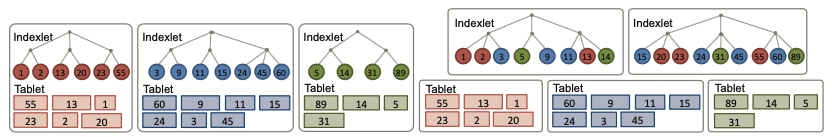
\includegraphics[width=\textwidth]{./figures/background/index_partitioning.png}

  \caption{Index partitioning schemes (temporary; borrowed)
  TODO: redo}

  \label{fig:index_partitioning}

\end{figure}

\bigskip
\noindent
\textbf{Partitioning Indexes by Document.}
In this approach, each partition is separate:
each partition maintains its own secondary indexes, covering only documents in that partition.

In a document-partitioned index (also known as a \textit{local index}),
each database write (adding, removing, or updating a document) is handled only by the partition that contains the
corresponding document.
Reading from a document-partitioned index requires a scatter/gather approach:
sending the query to all partitions and combining the returned results.
This can make index lookups quite expensive.
Even if index lookup requests are sent to partitions in parallel, response time depends from the latency of the slowest
index partition.

This approach is widely used: MongoDB, Riak \cite{riakv:secondaryindexes}, Cassandra \cite{cassandra:secondaryindexing}
Elasticsearch \cite{elastic:docrouting}, Solr \cite{solr:indexsharding}.

\bigskip
\noindent
\textbf{Partitioning Secondary Indexes by Term.}
An alternative approach is to construct a \textit{global index} that covers data in all partitions.
A global index, however, needs to be partitioned itself, as storing it on one node would likely become a bottleneck.

To partition a global index, the indexed terms can be used as the partition key (thus the term \textit{term-partitioned}
index).
Same as in base data partitioning, the index partitioning scheme can use the terms themselves, which can be useful for
range scans, or a the terms' hashes, which results to a more even load distribution.

The advantage of a term-partitioned index is that it can make reads more efficient:
rather than requiring a scatter/gather over all partitions, a lookup for a given term only needs to make a request to the
partition containing that term.
The downside of this approach is that writes are more complicated and slower:
a write to a single document may affect multiple partitions as the corresponding terms may correspond to multiple
different partitions.

DynamoDB supports both local and global secondary indexes \cite{dynamodb:secondaryindexes}.
Term-partitioned indexes have also been used in the research systems such as SLIK \cite{kejriwal:slik}
and Diff-Index \cite{tan:diffindex}.

\subsubsection{Query Planning and Execution}

Most non-relational databases have simple query models that do not support complex operations such as aggregation and
joins.
However, some document-oriented databases like MongoDB \cite{mongodb:joins}, RethinkDB \cite{rethinkdb:joins},
and CouchDB \cite{couchdb:joins} support join operations.
Query planning in NoSQL databases mainly deals with the database's distribution model:
a query execution plans consist of routing query requests to the appropriate data or index partitions.

\bibliographystyle{plainnat}
\bibliography{refs}
